% Latin.Science 2026 -- final full paper
% Uses the official event-supplied IEEEtran class and page artwork.
% The anonymous submission is preserved under submission_artifacts/.
\documentclass[a4paper,10pt,conference]{IEEEtran}

\usepackage{cite}
\usepackage[T1]{fontenc}
\usepackage[utf8]{inputenc}
\usepackage{graphicx}
\usepackage{booktabs}
\usepackage{tabularx}
\usepackage{array}
\usepackage[cmex10]{amsmath}
\usepackage{url}
\usepackage[hidelinks]{hyperref}
\hypersetup{
  pdftitle={Mapping AI in Scholarly Communication: Research Workflows, Named Models, and Governance},
  pdfauthor={Jedson Gabriel Ferreira de Paula; Joaquim de Oliveira Vieira; Willian Francisco da Silva; Claudio R. M. Mauricio},
  pdfkeywords={Bibliometrics; scholarly communication; generative artificial intelligence; research integrity; semantic embeddings; evidence synthesis},
  pdflang={en}
}
\usepackage{xcolor}
% Latin.Science 2026 page layout and event branding from the official template.
\usepackage[left=1.6cm,top=2cm,right=1.6cm,bottom=2.5cm,headheight=2cm,headsep=0cm,includehead]{geometry}
\usepackage{eso-pic}
\addtolength{\textheight}{-40.0pt}
\AddToShipoutPictureFG{%
  \AtPageUpperLeft{\raisebox{-\height}{
\includegraphics[width=\paperwidth]{headerimg.png}}}%
  \AtPageLowerLeft{
\includegraphics[width=\paperwidth]{footerimg.png}}%
}

\newcolumntype{Y}{>{\raggedright\arraybackslash}X}
% Generated by prepare_final.py.
\newcommand{\ValidationRhoT}{0.755}
\newcommand{\ValidationRhoG}{0.623}


\title{Mapping AI in Scholarly Communication:\\
Research Workflows, Named Models, and Governance}

\newif\iffinal
\finaltrue
\iffinal
\author{\IEEEauthorblockN{Jedson Gabriel Ferreira de Paula, Joaquim de Oliveira Vieira,\\
Willian Francisco da Silva, Claudio R. M. Mauricio}
\IEEEauthorblockA{Universidade Estadual do Oeste do Paran\'a (UNIOESTE)\\
Foz do Igua\c{c}u, Paran\'a, Brazil}}
\else
\author{}
\fi

\begin{document}
\maketitle

\begin{abstract}
AI is reshaping scholarly writing, peer review, evidence synthesis, and
institutional governance, but bibliometric mapping of these practices is
frustrated by broad database searches that return thousands of clinical,
engineering, and educational records. From 6,261 multi-source candidate records
in a locally preserved April 2026 snapshot, we applied documented scope rules
and retained 711 studies with publication years 2020--2026. Studies published
in 2026 provide provisional context. We positioned the retained studies on
two theory-guided semantic axes using prototype-anchored
BGE-M3 embeddings. Technological specificity (T) runs from generic AI to named
generative models; governance orientation (G) runs from workflow support to
integrity and institutional policy. A greedy variant-filtering procedure
selected prototypes to minimise the axis cosine (final cosine $=+0.0007$) with
leave-one-out stability $\rho \geq 0.98$. T and G were positively associated
after controlling for publication year (unstandardised $\beta=0.206$, 95\% CI
[0.119, 0.300]; partial $r=0.165$, $p<0.001$). Within a blinded, score-stratified
two-rater validation sample ($N=129$), unweighted Spearman correlations between
human ratings and final automated scores were \ValidationRhoT{}~(T) and
\ValidationRhoG{}~(G). Named-model specificity was weakly positively associated
with governance orientation, while workflow-support research remained present
across the technological-specificity range.
\end{abstract}

\renewcommand{\IEEEkeywordsname}{Keywords}
\begin{IEEEkeywords}
Bibliometrics; scholarly communication; generative artificial intelligence;
research integrity; semantic embeddings; evidence synthesis.
\end{IEEEkeywords}

\section{Introduction}

Generative AI has become a practical and debated component of academic work.
Tools based on large language models can assist with drafting, searching,
screening, summarising, and reviewing; the same tools have heightened debates
over fabricated references, disclosure, authorship, assessment, and research
integrity. These developments concern Latin.Science's interests in artificial
intelligence, governance, open technologies, and social impacts of technology.

The literature is difficult to characterise with a conventional keyword count.
Terms such as \emph{review}, \emph{screening}, \emph{writing}, and \emph{AI}
also occur in clinical AI, technical applications, and language-learning
studies. A broad retrieval therefore risks measuring the database's ambiguity
rather than the scholarly-communication field. Bibliometric work requires a
transparent definition of the population, documented data-processing
procedures, and
claims matched to the information that metadata and citations can support
\cite{pritchard1969,donthu2021,aria2017}.

This study addresses that problem by combining a documented scope-screening
procedure with
two interpretable semantic measurements. Rather than treating clusters from an
embedding space as discovered topics, we define two dimensions that correspond
to substantive questions. The first captures whether a paper concerns generic
AI or named generative models. The second distinguishes work centred on task support from work centred on governance, integrity, and institutional oversight.

We map a screened, multi-source corpus with publication years 2020--2026.
Five prototype abstracts per pole define each continuous axis. Variant selection
minimises prototype-level overlap while preserving leave-one-out stability.
We describe publication cohorts and estimate the association between
technological specificity and governance orientation.

We address three research questions:

\begin{enumerate}
  \item What publication-volume and semantic-composition patterns are observed
  across publication cohorts from 2020 to 2026 in this corpus snapshot?
  \item How are generic/named AI and workflow/governance orientations
  distributed in the retained literature?
  \item Is technological specificity associated with governance orientation
  after accounting for publication year?
\end{enumerate}

\section{Related Work}

Bibliometrics quantitatively studies bibliographic material to describe the
structure and evolution of a research field \cite{pritchard1969}. Contemporary
workflows combine transparent retrieval, deduplication, descriptive indicators,
and visual or network-based analyses \cite{donthu2021,aria2017}. The present
study uses reporting principles from PRISMA 2020 and PRISMA-S as transparency
guides for documenting identification and selection; it is not presented as a
systematic review or meta-analysis \cite{page2021,rethlefsen2021}.

Recent work on AI in scholarly communication has examined the rules and
practices surrounding authorship, disclosure, and editorial work. In a study of
300 leading journals, Lund and Naheem found that more than half had adopted
AI-authorship policies, but that the requirements differed by publisher and
discipline \cite{lund2024}. The ICMJE recommendations similarly place
responsibility for AI-assisted material on human authors and require disclosure
of the tool and its purpose; they also identify confidentiality as a constraint
on the use of AI in peer review \cite{icmje2026}. Policy responses at
universities have followed the same concerns without becoming uniform. Dabis and
Cs\'aki's analysis of policies from 30 universities identified accountability,
human oversight, transparency, and local implementation as recurring themes
\cite{dabis2024}.

The editorial-workflow literature gives a more concrete picture of both
potential and limitation. Checco \emph{et al.} developed and evaluated an
AI-assisted peer-review approach using 3,300 conference papers and reviews,
while noting risks of bias in automated quality judgements \cite{checco2021}.
More recently, Thakkar \emph{et al.} ran a randomised study of LLM feedback at
ICLR 2025 involving more than 20,000 reviews; reviewers who received feedback
produced more informative revisions \cite{thakkar2026}. Those results concern a
specific feedback intervention, not a general replacement for human review.
Integrity concerns are equally concrete. Walters and Wilder found fabricated
and erroneous entries in bibliographies generated by ChatGPT
\cite{walters2023}, and Koike \emph{et al.} showed that ordinary
task-related prompt constraints can materially change AI-text detector
performance \cite{koike2024}. Detection output should therefore not be treated
as proof of authorship.

Sentence embeddings provide a complementary tool for comparing abstracts at
scale. BGE-M3 supports multilingual and long-document retrieval settings, which
matters only if the embedded titles and abstracts are themselves multilingual
\cite{chen2024}. The search queries included English, Portuguese, and Spanish
terms, but all 711 retained titles and abstracts were English (by language
detection). The multilingual setting of BGE-M3 was therefore not needed; the
embeddings use only its English encoding. Embedding quality on general
benchmarks
does not, by itself, establish validity for a specific downstream construct;
construct-validity evidence must be gathered for the intended interpretation
\cite{fang2022}. For that reason, the semantic dimensions in this paper are
theory-guided and their interpretation is limited to the written poles and
observed patterns. A blinded two-rater human-validation study was conducted to
evaluate their convergent validity (Section~\ref{sec:validation-results}).

\section{Materials and Methods}
\label{sec:methods}

\subsection{Corpus construction and scope screening}

The starting corpus contained 6,261 articles and reviews with publication years
from 2020--2026, assembled from OpenAlex, Europe PMC, Scopus, Web of Science,
PubMed/MEDLINE, and BibTeX exports from ACM/IEEE-related searches. Records were
assembled in a locally preserved April 2026 snapshot. Local processing artifacts
are dated 10 April and manual exports include an early-11-April timestamp;
complete execution logs and record-level retrieval timestamps were not retained.
The supplement distinguishes preserved query specifications from execution logs.
Focused scope screening began on 8 August 2026; final anchor configuration and
analysis were refined during August. The corpus is therefore analysed as an
April 2026 multi-source snapshot rather than as an exhaustive census. Records
were deduplicated by
DOI and normalised title, and records without usable abstracts, retractions,
and records outside the time window were excluded before screening.

For the article population, we applied documented lexical-first scope rules to
title and abstract. Positive signals covered scholarly writing, publishing,
editorial and peer-review workflows, research integrity, AI-text detection,
evidence-synthesis automation, and AI literacy connected to higher education.
Negative signals covered clinical applications, engineering/industrial
applications, language learning, and school-level pedagogy. Conflicts were
routed through category-aware rules and a recorded review ledger. Cluster
membership was retained only as context and never determined inclusion.

The resulting ledger contained 711 included records, 5,542 excluded records,
and eight unresolved borderline records. Table~\ref{tab:selection-flow}
reports the complete processing and decision ledger. The
unresolved records were excluded from all analyses reported here. This is
single-reviewer, title-and-abstract screening; no inter-rater reliability is
claimed for this manuscript. Table~\ref{tab:corpus} gives the retained
corpus profile. The corpus is strongly concentrated in recent
publication years: 20 included records predate 2023 and 691 were published in
2023--2026. This distribution may reflect field emergence, retrieval coverage,
and database indexing; it is reported without trend modelling.

\begin{table}[!t]
\caption{Retained corpus after scope screening ($N=711$), by publication year and source. The 2026 count is provisional.}
\label{tab:corpus}
\centering
\footnotesize
\begin{tabular}{lr|lr}
\toprule
Year & $n$ & Source & $n$ \\
\midrule
2020 & 4 & Web of Science export & 533 \\
2021 & 6 & PubMed/MEDLINE export & 87 \\
2022 & 10 & Europe PMC & 40 \\
2023 & 99 & ACM/IEEE BibTeX export & 40 \\
2024 & 196 & Scopus & 9 \\
2025 & 314 & OpenAlex & 2 \\
2026 & 82 & & \\
\bottomrule
\end{tabular}
\par\vspace{3mm}
\begin{minipage}{0.90\columnwidth}
\raggedright\footnotesize Note: 2026 is a partial publication/indexing year and is used for context only. Counts describe the project corpus, not the annual population of all publications. After deduplication by DOI and normalised title, each record was assigned to a single source using the first-seen priority order in which databases were processed (Web of Science, PubMed/MEDLINE, Europe PMC, ACM/IEEE, Scopus, OpenAlex). The distribution therefore reflects both source coverage and this assignment rule.
\end{minipage}
\end{table}

\begin{table}[!t]
\caption{Corpus construction and final scope decisions.}
\label{tab:selection-flow}
\centering
\scriptsize
\begin{tabularx}{\columnwidth}{@{}Y r r r@{}}
\toprule
Step & Input & Removed & Retained \\
\midrule
\multicolumn{4}{@{}l}{\textit{Stage A. Broad-corpus assembly}} \\
Source assembly & 6,752 + 1,648 & -- & 8,400 \\
\addlinespace
Initial retrieval filters & 8,400 & $-$1,821 & 6,579 \\
Cleaning and embedding eligibility & 6,579 & $-$318 & 6,261 \\
\addlinespace
\multicolumn{4}{@{}l}{\textit{Stage B. Article-specific scope screen}} \\
Title-and-abstract scope screen & 6,261 & $-$5,542; $-$8 pending & \textbf{711} \\
\bottomrule
\end{tabularx}
\par\vspace{1mm}
\begin{minipage}{0.96\columnwidth}
\raggedright\footnotesize Note: Initial filters: no abstract 1,241; off-topic
title 150; weak alignment 228; low relevance 202. Cleaning: outside period 31;
retracted 20; off-topic 45; no usable embedding 222. Stage B is single-reviewer
title-and-abstract screening.
\end{minipage}
\end{table}

\subsection{Theory-guided semantic dimensions}

We used the 1,024-dimensional dense SentenceTransformer output of BGE-M3,
with L2-normalised document and prototype embeddings \cite{chen2024}.
The archived document representation joined the title, a period and space,
and the first 6,000 characters of the abstract. The stored model configuration
permits 8,192 tokens; longer inputs are truncated by the encoder. Each final
pole contains five controlled abstract prototypes. For axis $A\in\{T,G\}$,
let $\mathbf{p}_{A,\pm,j}$ be their normalised embeddings and define
\begin{align}
\mathbf{c}_{A,\pm}&=\tfrac{1}{5}\sum_{j=1}^{5}\mathbf{p}_{A,\pm,j},\\
\mathbf{m}_A&=(\mathbf{c}_{A,+}+\mathbf{c}_{A,-})/2,\\
\hat{\mathbf{u}}_A&=\frac{\mathbf{c}_{A,+}-\mathbf{c}_{A,-}}
{\|\mathbf{c}_{A,+}-\mathbf{c}_{A,-}\|_2},\\
s_A(\mathbf{v})&=(\mathbf{v}-\mathbf{m}_A)\cdot\hat{\mathbf{u}}_A.
\end{align}
Pole centroids are not re-normalised after averaging. Scores are continuous
projections, not probabilities or topic memberships. The supplement records
the checkpoint, preprocessing, available runtime information, and the command
that applies the exact final anchors to the preserved document embeddings.

\textbf{Technological specificity (T)} ranges from generic AI/ML without a
named generative model to papers in which a named model or model family (e.g.,
ChatGPT, GPT-4, Claude, Gemini, or LLaMA) is central. \textbf{Governance
orientation (G)} ranges from workflow support for writing, searching, review,
and synthesis to integrity, authorship, disclosure, policy, detection, and
institutional safeguards. Figure~\ref{fig:axis-instrument} illustrates the
construction and interpretation of a semantic axis using T as the running example.

\begin{figure*}[!t]
\centering
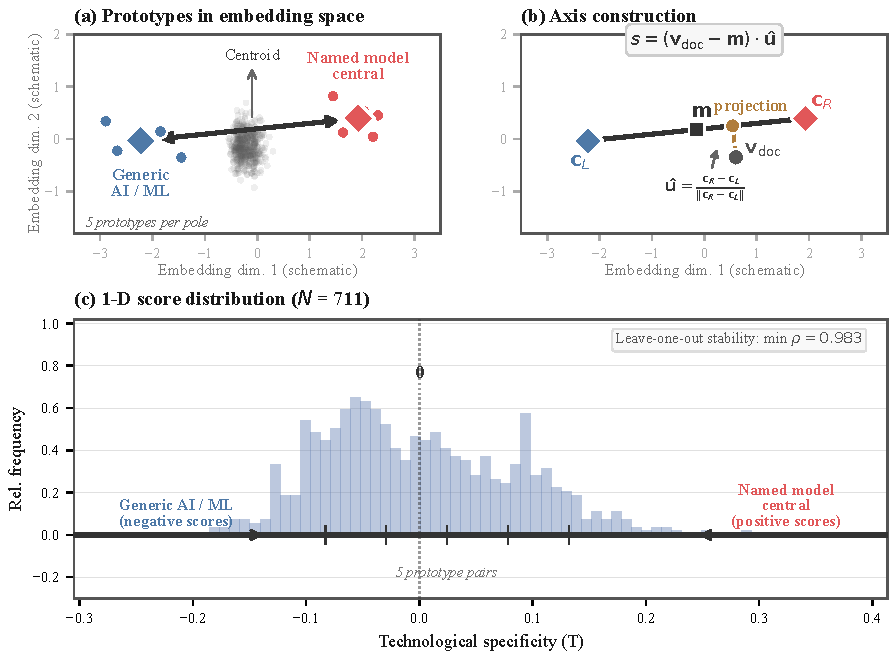
\includegraphics[width=\textwidth]{fig4_semantic_axis_instrument.pdf}
\caption{Construction and interpretation of a prototype-based semantic axis,
illustrated with the technological-specificity (T) dimension.
(a) Five prototype abstracts are written at each pole and embedded with
BGE-M3; their centroids define the axis direction.
(b) A document's score is its centred projection onto the unit vector between
centroids: $s = (\mathbf{v}_{\mathrm{doc}} - \mathbf{m}) \cdot \mathbf{\hat{u}}$.
(c) The resulting 1-D score distribution for the 711-record corpus, with
leave-one-out prototype stability (minimum $\rho=0.983$) confirming that the axis is
not determined by any single prototype.}
\label{fig:axis-instrument}
\end{figure*}

The 20 prototypes (5 per pole for each axis) anchor the measurement. Because
prototype wording can influence the resulting axis, each prototype was written
in several candidate variants. The final set was chosen by a greedy search:
each of the 20 positions takes the variant that minimises the absolute
T$\times$G axis cosine (the magnitude of the cosine between the two unit
vectors), subject to leave-one-prototype-out minimum Spearman $\rho \geq 0.97$
for both axes. The objective uses only the two anchor vectors. The stability
constraint uses corpus document-score ranks; neither the document-level T--G
association nor the human ratings are an objective or acceptance criterion
of the final selector. BGE-M3 embeddings for all
candidate prototypes were pre-computed, and the search continues until no
position can be improved.

The absolute T$\times$G axis cosine is $0.0007$ at the prototype level. Because
the objective minimised this quantity, near-orthogonality is a property of the
selection procedure rather than an independent finding. The document-level
association is estimated using the frozen final configuration; no coefficient
threshold was imposed by the final selector.
Leave-one-prototype-out stability is excellent for both axes (T min
$\rho=0.983$, G min $\rho=0.989$). The supplementary material records the
candidate variants, final configuration, and scoring procedure.

A near-zero prototype cosine does not guarantee independent document scores.
The Pearson correlation between T and G is $r=0.162$ in the retained corpus:
the dimensions are nearly orthogonal at the prototype level but weakly
correlated at the document level.

\subsection{Analysis plan}

We report annual counts and score distributions for four
completed calendar-year cohorts: 2020--2022 ($n=20$), 2023
($n=99$), 2024 ($n=196$), and 2025
($n=314$). The 2026 records ($n=82$) are shown for completeness but excluded
from comparisons between completed calendar-year cohorts because 2026 is
incomplete at the snapshot date. Completed calendar years do not imply
exhaustive database coverage. For
the principal association, we estimated an ordinary least-squares model of $G$
on $T$ and publication year, with sensitivity analyses excluding 2026 and
restricted to 2023--2025 with categorical year adjustment. Coefficient intervals
use 2,000 paired-record percentile bootstrap resamples; seeds for the principal
and sensitivity models are reported in the supplementary reproduction manifest
(S10). The partial correlation is calculated after residualising both T and G
on publication year.
These models describe association rather than causal effects.

\subsection{Human validation protocol}

A blinded 130-record sample was drawn from the included corpus, stratified by
publication-year cohort and the automated-score range available at sampling;
129 records had complete matched ratings on both axes. The sample and human
ratings were retained when final automated scores were reconciled. Because the sample was
stratified partly by automated-score range, the human--automated correlations
reported in Section~\ref{sec:validation-results} are correlations within the
stratified validation sample. Population inference would require appropriate
sampling weights and additional assumptions. Two independent raters scored T and G on anchored
1--5 Likert scales without seeing author,
venue, year, source, or automatic score. The
protocol specifies rank-order inter-rater consistency (Spearman), Spearman
association between the automated score and the mean of the two human scores,
calibration by score quintile, and bootstrap confidence intervals from 10,000
paired-record resamples; the seed is reported in S10. Final scores were matched to
the ratings through the preserved form-to-record crosswalk. Full validation results are reported in
Section~\ref{sec:validation-results}.

\section{Results}

\subsection{Concentration after 2023}

Figure~\ref{fig:temporal}(a) shows that the corpus contains four records dated 2020, 314 dated 2025, and 82
dated 2026. The 2026 count is partial and database-dependent. Annual counts are
not a complete census because database coverage, search histories, and indexing
lag differ by source. The clear post-2023 concentration is therefore
reported as a corpus-level pattern, not as an estimate of total annual
field output.

The corpus is not limited to higher-education commentary. It includes AI for
scientific writing and publishing, editorial workflows, research-integrity
policies, AI-text detection, and evidence-synthesis automation. This broader
but still delimited definition is important: an AI tool used to screen studies in
a health domain is in scope when the research object is the scholarly workflow,
whereas an AI system used to predict a clinical outcome is not.

\subsection{Semantic composition}

The April 2026 snapshot is concentrated in 2023--2025 (609/711 records). The
2020--2022 baseline contains 20 records and 2026 is partial; cohort
summaries therefore describe the retained corpus rather than estimate a stable
temporal trend. In the pooled 2020--2022 baseline, median T was -0.067 and
median G was -0.111. Across the completed annual cohorts from 2023 to 2025,
median T was 0.026 in 2023,
0.007 in 2024, and -0.018 in 2025; median G was 0.081, 0.047, and 0.033,
respectively. Figures~\ref{fig:temporal}(b) and \ref{fig:temporal}(c) show
the overlapping cohort distributions of T and G. These distributions do not establish a smooth linear
change over publication years.

\begin{figure}[!t]
\centering
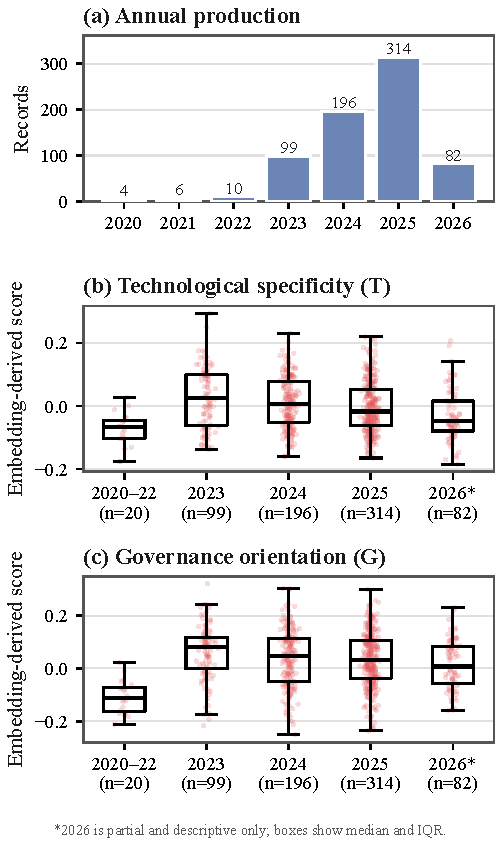
\includegraphics[width=\columnwidth]{fig1_temporal_production_and_distributions.pdf}
\caption{Retained records by publication year and T/G score distributions
($N=711$). Distribution cohorts are 2020--2022 ($n=20$), 2023 ($n=99$),
2024 ($n=196$), 2025 ($n=314$), and incomplete 2026 ($n=82$).
Boxes show medians and interquartile ranges; points show individual records.
The 2026 cohort is descriptive only. Counts describe the April 2026 corpus
snapshot, not exhaustive annual field output. Inputs and production dates
are recorded in supplementary manifest S10.}
\label{fig:temporal}
\end{figure}

\subsection{Named-model specificity and governance orientation}

Technological specificity and governance orientation are positively
associated in the retained corpus (Figure~\ref{fig:tg}). Controlling for
publication year (encoded as a continuous integer), T predicted G
(unstandardised $\beta=0.206$, 95\% CI [0.119, 0.300]). The partial
correlation was $r=0.165$ ($p=1.1\times 10^{-5}$); the model explained
2.8\% of G's variance, compared with 0.07\% for year alone. The unique
effect of T was small ($f^2=0.028$). The association remained positive
when 2026 was excluded ($\beta=0.234$, 95\% CI [0.140, 0.324]) and in the
complete 2023--2025 cohorts with categorical year adjustment ($\beta=0.187$,
95\% CI [0.095, 0.284]). This cross-sectional association between
embedding-derived indicators does not imply that using a named model causes
governance concern.

One reading of this pattern is: papers that make
ChatGPT or another named model central more often also address disclosure,
integrity, institutional policy, or safeguards. Workflow-oriented work remains
present across the score range and should not be cast as displaced by governance
research.

\begin{figure}[!t]
\centering
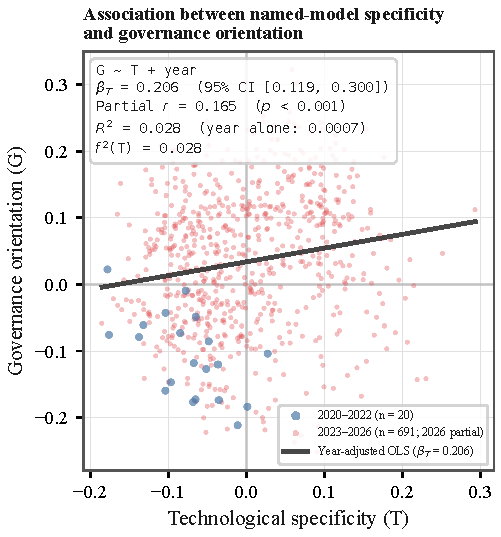
\includegraphics[width=\columnwidth]{fig2_t_vs_g_scatter.pdf}
\caption{Final T and G scores for all 711 retained records. Higher T indicates
greater named-model specificity; higher G indicates greater governance
orientation. Colours distinguish 2020--2022 ($n=20$) from 2023--2026
($n=691$, including incomplete 2026). The line is the fit from
$G\sim T+\text{publication year}$ evaluated at mean publication year.
The coefficient interval is a 95\% percentile bootstrap interval;
no uncertainty band is plotted. Inputs and production dates are in S10.}
\label{fig:tg}
\end{figure}

\subsection{Human-validation results}
\label{sec:validation-results}
% Generated from final scores and verified human ratings by prepare_final.py.
Two blinded raters independently assessed 130 sampled records; 129 had complete matched ratings on both axes.
All automated scores below use the frozen final anchors and the same document scores as the principal analysis.

\textit{Inter-rater rank consistency.} Spearman's $\rho$ measures rank association rather than exact agreement; quadratic-weighted $\kappa$ is reported alongside it.
For technological specificity (T), inter-rater Spearman $\rho=0.755$ (95\% bootstrap CI [0.659, 0.834], $p<0.001$), Pearson $r=0.750$, and quadratic-weighted $\kappa=0.631$.
For governance orientation (G), inter-rater Spearman $\rho=0.806$ (95\% bootstrap CI [0.722, 0.871], $p<0.001$), Pearson $r=0.823$, and quadratic-weighted $\kappa=0.805$.

\textit{Convergence with final automated scores.} The reference was the mean of the two human ratings.
For T, human--automated Spearman $\rho=0.755$ (95\% bootstrap CI [0.663, 0.821], $p<0.001$; Pearson $r=0.775$). Per-rater Spearman correlations were 0.607 and 0.783.
For G, human--automated Spearman $\rho=0.623$ (95\% bootstrap CI [0.490, 0.732], $p<0.001$; Pearson $r=0.644$). Per-rater Spearman correlations were 0.516 and 0.656.

\textit{Quintile calibration.} Records were grouped into quintiles of the final automated scores within the validation sample.
For T, mean human scores across quintiles 1--5 were 1.73, 1.79, 2.76, 3.56, and 4.35.
For G, mean human scores across quintiles 1--5 were 1.42, 3.33, 3.26, 4.19, and 4.38.
Human scores rose overall, but the quintile means were not strictly monotonic for both axes.

These unweighted results describe the score-stratified validation sample. They support convergence with the judgements of two human readers; they do not estimate population-wide validity or establish validity for other corpora.


\section{Discussion}

The weak association between named-model specificity and governance orientation
is plausible in scholarly communication: institutions and publishers must
address authorship, disclosure, assessment, and reliability as models enter
writing and review workflows.

Scope definition is essential. The broad AI search returned thousands of
clinical, engineering, and teaching records. The documented screening procedure
and preserved internal ledger define the boundary around scholarly workflows
and retain unresolved cases outside the analytical corpus.

The semantic axes complement keyword co-occurrence, bibliographic coupling,
and co-citation methods by positioning records on theory-guided dimensions.
Findings are constrained to the constructs represented by the chosen poles.

Interpretation is constrained by several features of the design. The corpus is
not an exhaustive census and is dominated by recent records and Web of Science
exports. Abstract-based screening cannot always distinguish a scholarly task
from an incidental method reference.
Prototype wording and selection affect the measurement. The near-zero axis
cosine is an optimisation result; LOO stability concerns robustness to individual
anchors. Neither establishes construct validity. Human validation supplies
additional evidence, but its unweighted correlations describe the deliberately
stratified sample. Corpus coverage and the two-rater design limit generalisation.

The publication supplement provides exact prototype texts, de-identified
derived scores, matched validation ratings, and statistical reproduction code.
Future work can release additional screening material where source terms permit,
compare alternative embedding models, and analyse changes as the 2026 literature
matures.

\raggedbottom
\section{Conclusion}

This paper maps 711 studies on AI in scholarly communication and research
workflows with publication years 2020--2026 in a locally preserved April 2026
snapshot. The 2026 cohort is incomplete and supplies descriptive context;
comparisons between completed calendar-year cohorts exclude it.
The screened literature is concentrated in 2023--2025 and
shows a positive year-adjusted association between named-model specificity and
governance orientation. The result is best read as a descriptive map of
a developing field rather than a causal account or a replacement for human judgement.
By making scope rules and semantic anchors explicit, the approach supports
evidence-based discussion of AI's practical and institutional roles in research.

\section*{Declaration on Use of Generative Artificial Intelligence}
Claude Code using a DeepSeek model assisted code development and data processing
during analysis. NotebookLM assisted background research during study preparation.
ChatGPT assisted manuscript review, statistical consistency checks, and revision
during writing and final preparation. Some candidate prototype texts were drafted
or revised with generative-AI tools as measurement inputs. Exact assistance-model
versions and candidate-by-candidate generation records were not retained.
The authors reviewed the final anchors, data-selection decisions, statistical
outputs, cited sources, and manuscript, and take responsibility for the work.

\section*{Code and Data Availability}
The camera-ready paper, source files, and individually browsable reproduction
materials are available in the \href{https://github.com/ShutDownMan/ai-bibliometrics/tree/latinscience2026-v1.0.0/paper/latinscience2026}{versioned public release}.
The included derived tables and scripts reproduce the reported statistics and
figures. Source database records and document embeddings are omitted under
their access terms; recomputing document scores requires those preserved inputs.
Historical retrieval timestamps and embedding-runtime versions were not recorded.

% Balance the final columns using IEEEtran's built-in reference trigger.
\IEEEtriggeratref{1}
\IEEEtriggercmd{\enlargethispage{-1.5in}}
\begin{thebibliography}{00}

\bibitem{pritchard1969}
A. Pritchard, ``Statistical bibliography or bibliometrics?,'' \emph{Journal of
Documentation}, vol. 25, no. 4, pp. 348--349, 1969.

\bibitem{donthu2021}
N. Donthu, S. Kumar, D. Mukherjee, N. Pandey, and W. M. Lim, ``How to conduct a
bibliometric analysis: An overview and guidelines,'' \emph{Journal of Business
Research}, vol. 133, pp. 285--296, 2021, doi: 10.1016/j.jbusres.2021.04.070.

\bibitem{aria2017}
M. Aria and C. Cuccurullo, ``bibliometrix: An R-tool for comprehensive science
mapping analysis,'' \emph{Journal of Informetrics}, vol. 11, no. 4, pp.
959--975, 2017, doi: 10.1016/j.joi.2017.08.007.

\bibitem{page2021}
M. J. Page \emph{et al.}, ``The PRISMA 2020 statement: an updated guideline
for reporting systematic reviews,'' \emph{BMJ}, vol. 372, p. n71, 2021,
doi: 10.1136/bmj.n71.

\bibitem{rethlefsen2021}
M. L. Rethlefsen \emph{et al.}, ``PRISMA-S: an extension to the PRISMA
statement for reporting literature searches in systematic reviews,''
\emph{Systematic Reviews}, vol. 10, p. 39, 2021,
doi: 10.1186/s13643-020-01542-z.

\bibitem{chen2024}
J. Chen, S. Xiao, P. Zhang, K. Luo, D. Lian, and Z. Liu, ``BGE M3-Embedding:
Multi-lingual, multi-functionality, multi-granularity text embeddings through
self-knowledge distillation,'' arXiv:2402.03216, 2024.

\bibitem{fang2022}
Q. Fang, D. Nguyen, and D. L. Oberski, ``Evaluating the construct validity of
text embeddings with application to survey questions,'' \emph{EPJ Data Science},
vol. 11, art. no. 39, 2022, doi: 10.1140/epjds/s13688-022-00353-7.

\bibitem{lund2024}
B. D. Lund and K. T. Naheem, ``Can ChatGPT be an author? A study of artificial
intelligence authorship policies in top academic journals,'' \emph{Learned
Publishing}, vol. 37, no. 1, pp. 13--21, 2024,
doi: 10.1002/leap.1582.

\bibitem{icmje2026}
International Committee of Medical Journal Editors, ``Use of artificial
intelligence in publishing,'' \emph{ICMJE Recommendations}, 2026. [Online].
Available: \url{https://www.icmje.org/recommendations/browse/artificial-intelligence/}.
[Accessed: Aug. 8, 2026].

\bibitem{dabis2024}
A. Dabis and C. Cs\'aki, ``AI and ethics: Investigating the first policy
responses of higher education institutions to the challenge of generative AI,''
\emph{Humanities and Social Sciences Communications}, vol. 11, art. no. 1006,
2024, doi: 10.1057/s41599-024-03526-z.

\bibitem{checco2021}
A. Checco, L. Bracciale, P. Loreti, S. Pinfield, and G. Bianchi,
``AI-assisted peer review,'' \emph{Humanities and Social Sciences
Communications}, vol. 8, art. no. 25, 2021,
doi: 10.1057/s41599-020-00703-8.

\bibitem{thakkar2026}
N. Thakkar \emph{et al.}, ``A large-scale randomized study of large language
model feedback in peer review,'' \emph{Nature Machine Intelligence}, vol. 8,
pp. 326--336, 2026, doi: 10.1038/s42256-026-01188-x.

\bibitem{walters2023}
W. H. Walters and E. I. Wilder, ``Fabrication and errors in the bibliographic
citations generated by ChatGPT,'' \emph{Scientific Reports}, vol. 13, art. no.
14045, 2023, doi: 10.1038/s41598-023-41032-5.

\bibitem{koike2024}
R. Koike, M. Kaneko, and N. Okazaki, ``How you prompt matters! Even
task-oriented constraints in instructions affect LLM-generated text detection,''
in \emph{Findings of the Association for Computational Linguistics: EMNLP
2024}, 2024, pp. 14384--14395, doi: 10.18653/v1/2024.findings-emnlp.841.

\end{thebibliography}

\end{document}
